% This is samplepaper.tex, a sample chapter demonstrating the
% LLNCS macro package for Springer Computer Science proceedings;
% Version 2.20 of 2017/10/04
%
\documentclass[runningheads]{llncs}
%
\usepackage{amsmath}
\usepackage{graphicx}
% Used for displaying a sample figure. If possible, figure files should
% be included in EPS format.
%
% If you use the hyperref package, please uncomment the following line
% to display URLs in blue roman font according to Springer's eBook style:
% \renewcommand\UrlFont{\color{blue}\rmfamily}

\begin{document}
%
\title{An Evaluation of Uninformed and Informed Search Algorithms on the $k$-puzzle Problem}
\subtitle{AY19/20 Semester 2 CS3243 Project 1, Group 37}
%
\titlerunning{Search Algorithms on the $k$-puzzle Problem}
% If the paper title is too long for the running head, you can set
% an abbreviated paper title here
%
\author{Lim Fong Yuan \and
Zhuang Xinjie \and
Otto Alexander Sutianto \and
Mario Lorenzo}
%
\authorrunning{Lim et al.}
% First names are abbreviated in the running head.
% If there are more than two authors, 'et al.' is used.
%
\institute{School of Computing, National University of Singapore% \and
%Springer Heidelberg, Tiergartenstr. 17, 69121 Heidelberg, Germany
%\email{lncs@springer.com}\\
%\url{http://www.springer.com/gp/computer-science/lncs} \and
%ABC Institute, Rupert-Karls-University Heidelberg, Heidelberg, Germany\\
%\email{\{abc,lncs\}@uni-heidelberg.de}
}
%
\maketitle              % typeset the header of the contribution
%
%\begin{abstract}
%The abstract should briefly summarize the contents of the paper in
%150--250 words.

%\keywords{First keyword  \and Second keyword \and Another keyword.}
%\end{abstract}
%
%
%
\section{Problem Specification}
%\begin{enumerate}
%\item A suitable representation should be specified to define the problem
%\item It should facilitate the formulation of search-based solutions
%\end{enumerate}

Fix $n \in \bbbz_{\geq 2}$. Let $k = n^2 -1$.
A valid state $v$ is a $n \times n$ array with the entries $v_{(x,y)}$ containing a permutation of the integers $[0,k]$. $V$ is the set of valid states.
Each valid state has a unique coordinate $e = (x_e,y_e)$ such that $v_e = 0$. Call $v_e$ the empty cell of $v$.
An initial state $s$ is a valid state with $e = (n,n)$.
The goal state $g$ is where $g_{(x,y)} = (x-1)n+y$ for all $(x,y) \in (\bbbz_{[1,n]})^2$, except for $g_{(n,n)}$ which is $0$.
Let $A = \{\texttt{up}=(-1,0),\texttt{down}=(1,0),\texttt{left}=(0,-1),\texttt{right}=(0,1)\}$ be the set of actions.
The transition function $T: V \times A \to V$ is where $T(v,a) = v'$ with $v'$ being identical to $v$ except with $(v'_{e-a},v'_e) = (v_e,v_{e-a})$.% (Invalid output states are rejected.)

The problem is to determine if $g$ is reachable from a given initial state $s$, and if so, specify a sequence of actions $p \in A^\ast$ that leads from $s$ to $g$.



%Please try to avoid rasterized images for line-art diagrams and schemas. Whenever possible, use vector graphics instead (see Fig.~\ref{fig1}).
\begin{figure}
	\centering
	%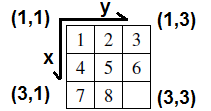
\includegraphics[width=\textwidth]{coord_system.png}
	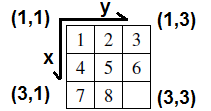
\includegraphics{coord_system.png}
	\caption{The coordinate system and the goal state, in the case of $n=3$.} \label{fig:coordsystem}
\end{figure}



\section{Technical Analysis}
\subsection{[Uninformed Search]}
\subsubsection{Correctness}
[BLAH]

%

%\noindent Displayed equations are centered and set on a separate line.
%\begin{equation}
%x + y = z
%\end{equation}

%\begin{theorem}
%This is a sample theorem. The run-in heading is set in bold, while the following text appears in italics. Definitions, lemmas, propositions, and corollaries are styled the same way.
%\end{theorem}
%
% the environments 'definition', 'lemma', 'proposition', 'corollary',
% 'remark', and 'example' are defined in the LLNCS documentclass as well.
%
%\begin{proof}
%Proofs, examples, and remarks have the initial word in italics, while the following text appears in normal font.
%\end{proof}

\subsubsection{Efficiency}
Given any valid state, there are up to $|A|=4$ possible actions. However, the initial state only has 2 possible actions, and every state thereafter has an action that backtracks and can thus be discounted, thus the maximum branching factor $b$ of the problem space is $|A|-1=3$. // This algorithm thus has $O(3^d)$ time and $O(3^d)$ space complexity.

\subsection{[Informed Search]}
\subsubsection{Correctness}
[BLAH]

\subsubsection{Efficiency}
[BLAH]

\subsubsection{Heuristics}
\paragraph{Heu1}
The 3 heuristics should be distinct and non-trivial; for example, your heuristic should not be a constant, a simple linear transformation of other heuristics, or any simple function of another heuristic like a square root of another

Consistency/Admissibility: Your heuristic must be provably admissible, or (preferably) consistent. In either case you must formally prove this property. Note that consistency implies admissibility but not the other way around. Thus, if you show admissibility, you should provide a (preferably simple) counterexample where your heuristic violates consistency.

\paragraph{Heu2}
[desc]

\paragraph{Heu3}
[desc]



\section{Experimental Setup}
\begin{enumerate}
\item The goal of the experiments should be defined (including a rationale for the chosen algorithms and heuristics), and in particular the metrics designed/used should be justified
\item The entire experimental process should be clearly defined such that the experiments may be replicated
\end{enumerate}

\begin{table}
\caption{Table captions should be placed above the tables.}\label{tab1}
\begin{tabular}{|l|l|l|}
\hline
Heading level &  Example & Font size and style\\
\hline
Title (centered) &  {\Large\bfseries Lecture Notes} & 14 point, bold\\
1st-level heading &  {\large\bfseries 1 Introduction} & 12 point, bold\\
2nd-level heading & {\bfseries 2.1 Printing Area} & 10 point, bold\\
3rd-level heading & {\bfseries Run-in Heading in Bold.} Text follows & 10 point, bold\\
4th-level heading & {\itshape Lowest Level Heading.} Text follows & 10 point, italic\\
\hline
\end{tabular}
\end{table}



\section{Results and Discussion}
\begin{enumerate}
\item The results from your experimentation should be clearly summarised (you may include more detailed results in an Appendix,
which would not count towards the given page limit – these will only be optionally viewed at the markers’ discretion)
\item A concise discussion comparing the theoretical analysis and empirical results should be given to elucidate the effectiveness and efficiency of your implementations
\end{enumerate}



%Multiple citations: \cite{ref_article1,ref_book1,ref_proc1,ref_url1}

%\cite{Perlin85}
%
% ---- Bibliography ----
%
% BibTeX users should specify bibliography style 'splncs04'.
% References will then be sorted and formatted in the correct style.
%
\bibliographystyle{splncs04}
%\bibliography{mybib}

\end{document}
